\documentclass[10pt,a4paper]{article}
\usepackage[utf8]{inputenc}
\usepackage[T1]{fontenc}
\usepackage[english]{babel}


\usepackage[margin=2.5cm]{geometry}
\usepackage[parfill]{parskip}
\usepackage{fix-cm}
\usepackage{pdfpages}
\usepackage[hidelinks]{hyperref}
\usepackage{graphicx, float}

\usepackage{setspace}
\onehalfspacing

% paths used for images
\graphicspath{{img/}}


\author{Christoffer Fridlund, Lasse Lybeck}
\title{Kimble AI competition}


\begin{document}


\maketitle

\tableofcontents


\section{Introduction}

Kimble (also known as Trouble) is a game where players compete to be the first to send four pieces all the way around the game board. The aim of this competition is to program an AI (Artificial Intelligence) to play this game and compete against other AIs (or possibly human players).

The rules of the game are covered in section \ref{sec:rules}. The technincal specifications of the competition can be found in section \ref{sec:tech-specs}. Other information (including information about the template Java-project) can be found in section \ref{sec:other-info}.


\section{Game rules}
\label{sec:rules}

\subsection{Game setup}

All participating players select one of the avaiable colors. After this, all the players place their four (4) pieces into their home squares.

\subsection{Who starts?}

The player to begin the actual game is chosen through a die roll competition. All players roll the die and the highest value gets to start. If there are two or more equally high die rolls, the ones who rolled these roll again until only one has the highest die value. The turn then moves clockwise.

\textbf{Example:}

\begin{tabular}{c c}
	Player & Die Roll \\
	A & 3 \\
	B & 4 \\
	C & 2 \\
	D & 4
\end{tabular}

Then player B and player D have to roll again to see who gets the higher value.

\subsection{How to move a piece}

Each turn the player in turn rolls the die. The player may then move one piece according to the following rules. If the player rolled a six (6), then the player is awarded an extra turn. If no move is possible or only optional moves are possible and the player chooses to pass, the turn goes to the next player.

\subsubsection{Moving out of Home}

If the player in turn rolls a one (1) or a six (6) he/she may move one piece from the home square to the start square (given there are still pieces left in the home squares). However, the move cannot be made if the start square is already occupied by one of the players own pieces. If the start square is occupied by one of some other players pieces the piece can be eaten as explained in section \ref{sec:eat}.

\subsubsection{Move in the Field}

After rolling the die a piece on the field can be moved clockwise around the table a number of steps equal to the die roll. If there is however a players own piece on the destination square the move cannot be made. If some other player's piece occupies the destination square it can be eaten as described in section \ref{sec:eat}. An example of a move can be found in figure \ref{fig:move-normal}.

\begin{figure}[H]
\begin{center}
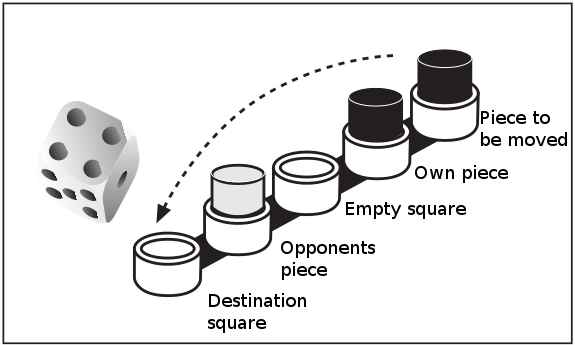
\includegraphics[width=.4\linewidth]{move-1.png}
\end{center}
\caption{Example of a normal move.}
\label{fig:move-normal}
\end{figure}

\subsubsection{Eating}
\label{sec:eat}

If the destination square of the move is occupied by piece belonging to another player the piece can be eaten. The move is made as normal, and the eaten piece is moved back to its home squares. An example can be found in figure \ref{fig:move-eat}.

\begin{figure}[H]
\begin{center}
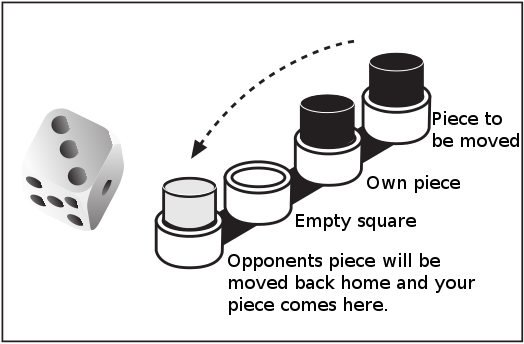
\includegraphics[width=.4\linewidth]{move-2.png}
\end{center}
\caption{Example of an eating move.}
\label{fig:move-eat}
\end{figure}

\subsubsection{Move into and in the Goal}

When a piece has traveled around the game board and would with a move pass the player's own start square it can be moved into the goal area. The piece moves as in the field in the goal, but can bounce back from the last square. If the piece is moved to the last goal square and there are still remaining steps to be taken the piece starts moving back toward the start of the goal squares. The piece may however not be moved back into the field.

A piece that occupies a goal square may also be moved. This is however an \textbf{optional move}, which means that if the only possible move for a player is to move a piece already occupying a goal square, the turn may be passed without moving. This is the only situation where a player may choose not to move, altough there are legal moves available. When moving a piece from a goal square it is first moved away from the field, and may then be bounced off the last square as described above. As usual, the piece may not leave the goal squares and head back into the field.

An example of a move into the goal can be found in figure \ref{fig:move-goal}. In the figure the same result would also come if the die roll would have been a 5, as the piece from the field would have bounced from the last square back to square number 3. Another legal move (although in this case a stupid move) would be to move the piece in square 2. The piece would also land in square 3, after bouncing back from the last goal square.

\begin{figure}[H]
\begin{center}
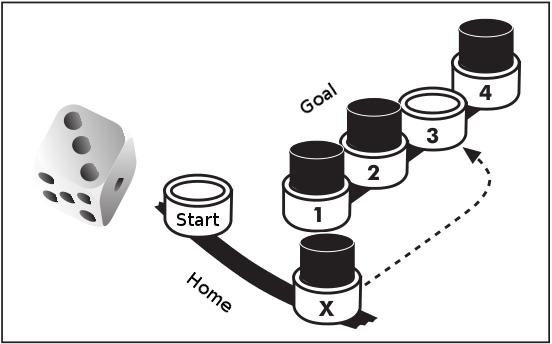
\includegraphics[width=.4\linewidth]{move-3.png}
\end{center}
\caption{Example of a move into the goal.}
\label{fig:move-goal}
\end{figure}

\subsection{Who wins?}

The one to first get all the pieces from the playing board into the goal wins.



\section{Technical specifications}
\label{sec:tech-specs}

% Technincal specs here.

In the competition there'll be \textbf{four (4)} players competing against each other with \textbf{four (4)} pieces each.

The game is run like a server and the AIs runs as clients connected to the server.



\section{Other information}
\label{sec:other-info}

% Other info here. This includes info about the template NetBeans-project.

It's strongly recommended that you check out all the template classes found in the KimbleAI project. They are done to be as simple as possible for you to use.

\subsection{Test Running Your AI}

The server is configured to start the clients as own processes by running the \textit{kimbleai.TournamentMain} class (java -cp YourJar.jar kimbleai/TournamentMain) this means that you \textbf{SHALL NOT} change or move this class. However there is one exception, if you change the name of \textit{yourpackage}, make sure that the \textit{kimbleai.TournamentMain} points to the new \textit{yourpackage.Main.startClient(host, port)} method (this method is used to start your implemented AI).

The clients (jar files) started are the ones specified in the implementation of the \textit{LoadClientsInterface}, as default are four instances of YourJar.jar run (see the comments and code in \textit{templates.LoadClients}). To run multiple different AIs you should build them all into separate jars! This is easiest achieved by maintaining multiple copies of the project one for each of your AIs you make and then just press the Clean-Build button in Netbeans. Another simple way (but riskier) is to rename the built jar before building again.

%\vspace{0.3cm}

\subsection{Runtime Parameters}

There are some parameters in the \textit{yourpackage.Main} to modify the server on startup:
\begin{itemize}

\item boolean USE\_GUI - make the gui visible or hidden. When it is visible the game is run approximately at 60 frames per second. When it is hidden the game runs as fast as possible.

\item boolean USE\_LOGGER - logs each run as a separate json file. The log is later possible to replay through a Playback application.

\item boolean USE\_HUD - (still wondering if this is necessary)

\item String HOST\_ADDRESS - the url in text form to the server. This is for now run on the 'localhost' (later it'll be possible to run over networks as well).

\item int PORT - the port on the HOST\_ADDRESS to connect to. This allows for multiple servers to be run on the same machines (as long as they have different ports).

\end{itemize}

The sample code is heavily commented and should be sufficient to get you going.

\subsection{External files or folders}

If you are in need of external files, you can either pack them inside your jar and load them with the \textit{getClass().getResouce()} methods or make sure that your external files are inside a unique directory (so they don't interfere with other projects' resources).


\subsection{Sending in Your Contribution}

%\vspace{0.5cm}

WHEN SENDING IN YOUR YourJar.jar TO US IT HAS TO HAVE A UNIQUE NAME (ALL AIs ARE SAVED IN THE SAME DIRECTORY). IT'S ALSO BASED ON THIS NAME YOU FIND YOURSELF IN THE COMPETITION RANKINGS.

%\vspace{0.5cm}



\end{document}